\documentclass[12pt, titlepage]{article}

\usepackage{fullpage}
\usepackage[round]{natbib}
\usepackage{multirow}
\usepackage{booktabs}
\usepackage{tabularx}
\usepackage{graphicx}
\usepackage{float}
\usepackage{hyperref}
\usepackage{helvet}
\usepackage[letterpaper, portrait, margin=1in]{geometry}
\hypersetup{
    colorlinks,
    citecolor=blue,
    filecolor=black,
    linkcolor=red,
    urlcolor=blue
}
\renewcommand{\familydefault}{\sfdefault}
%% Comments

\usepackage{color}

\newif\ifcomments\commentstrue %displays comments
%\newif\ifcomments\commentsfalse %so that comments do not display

\ifcomments
\newcommand{\authornote}[3]{\textcolor{#1}{[#3 ---#2]}}
\newcommand{\todo}[1]{\textcolor{red}{[TODO: #1]}}
\else
\newcommand{\authornote}[3]{}
\newcommand{\todo}[1]{}
\fi

\newcommand{\wss}[1]{\authornote{blue}{SS}{#1}} 
\newcommand{\plt}[1]{\authornote{magenta}{TPLT}{#1}} %For explanation of the template
\newcommand{\an}[1]{\authornote{cyan}{Author}{#1}}

%% Common Parts

\newcommand{\progname}{ProgName} % PUT YOUR PROGRAM NAME HERE
\newcommand{\authname}{Team \#, Team Name
\\ Student 1 name and macid
\\ Student 2 name and macid
\\ Student 3 name and macid
\\ Student 4 name and macid} % AUTHOR NAMES                  

\usepackage{hyperref}
    \hypersetup{colorlinks=true, linkcolor=blue, citecolor=blue, filecolor=blue,
                urlcolor=blue, unicode=false}
    \urlstyle{same}
                                


\newcounter{acnum}
\newcommand{\actheacnum}{AC\theacnum}
\newcommand{\acref}[1]{AC\ref{#1}}

\newcounter{ucnum}
\newcommand{\uctheucnum}{UC\theucnum}
\newcommand{\uref}[1]{UC\ref{#1}}

\newcounter{mnum}
\newcommand{\mthemnum}{M\themnum}
\newcommand{\mref}[1]{M\ref{#1}}

\begin{document}

\title{Module Guide for \progname{}}
\author{\authname}
\date{\today}

\maketitle

\pagenumbering{roman}

\section{Revision History}

\begin{tabularx}{\textwidth}{p{3cm}p{2cm}X}
  \toprule {\bf Date} & {\bf Version} & {\bf Notes} \\
  \midrule
  Date 1              & 1.0           & Notes       \\
  Date 2              & 1.1           & Notes       \\
  \bottomrule
\end{tabularx}

\newpage

\section{Reference Material}

This section records information for easy reference.

\subsection{Abbreviations and Acronyms}

\renewcommand{\arraystretch}{1.2}
\begin{tabular}{l l}
  \toprule
  \textbf{symbol} & \textbf{description}                \\
  \midrule
  AC              & Anticipated Change                  \\
  DAG             & Directed Acyclic Graph              \\
  M               & Module                              \\
  MG              & Module Guide                        \\
  OS              & Operating System                    \\
  R               & Requirement                         \\
  SC              & Scientific Computing                \\
  SRS             & Software Requirements Specification \\
  \progname       & Explanation of program name         \\
  UC              & Unlikely Change                     \\
  \bottomrule
\end{tabular}\\

\newpage

\tableofcontents

\listoftables

\listoffigures

\newpage

\pagenumbering{arabic}

\section{Introduction}

This document serves as the module guide for the system currently in development by Back End Developers. It will decompose the system into modules; detailing the purpose of each individual module of the system, what resources are necessary to fulfill the requirements of each module, and the interactions between said modules. In addition, this document will list the anticipated and unlikely changes expected for the system, and the relevant traceability matrices between related components. \\

This document has been written to address the needs of a wide audience. It is intended to help on-board new members joining the project by providing them with a structured breakdown of the project in its intended state, and is intended to provide a reference document to the engineers who are responsible for maintenance of the system should they feel that they need to make any necessary changes. In addition, it is intended to be read by the designers of the system itself; to give them the ability to have a big-picture overview of the system that they are working on. After a thorough read-through of this document, a reader with a reasonable amount of background knowledge (see document from before) should be able to recreate the functionality of each module, their interactions with each other, and therefore the system as a whole.\\

For this document to fulfill all of these requirements specified above is a difficult task, and the content of it is likely unable to capture 100\% of the information necessary to fulfill its goals to perfection. It should be obvious that engineers are by no means omniscient, not even regarding the systems that they design themselves. However, the authors of this document will still attempt to cover the relevant content in a digestible and comprehensive way, and thank the reader for their patience and good will.\\

\section{Anticipated and Unlikely Changes} \label{SecChange}

This section lists possible changes to the system. According to the likeliness
of the change, the possible changes are classified into two
categories. Anticipated changes are listed in Section \ref{SecAchange}, and
unlikely changes are listed in Section \ref{SecUchange}.

\subsection{Anticipated Changes} \label{SecAchange}

Anticipated changes are the source of the information that is to be hidden
inside the modules. Ideally, changing one of the anticipated changes will only
require changing the one module that hides the associated decision. The approach
adapted here is called design for
change.

\begin{description}
  \item[\refstepcounter{acnum} \actheacnum \label{acHardware}:] The specific
    hardware on which the software is running.
  \item[\refstepcounter{acnum} \actheacnum \label{acInput}:] The format of the
    initial input data.
\end{description}

\subsection{Unlikely Changes} \label{SecUchange}

The module design should be as general as possible. However, a general system is
more complex. Sometimes this complexity is not necessary. Fixing some design
decisions at the system architecture stage can simplify the software design. If
these decision should later need to be changed, then many parts of the design
will potentially need to be modified. Hence, it is not intended that these
decisions will be changed.

\begin{description}
  \item[\refstepcounter{ucnum} \uctheucnum \label{ucIO}:] Input/Output devices
    (Input: File and/or Keyboard, Output: File, Memory, and/or Screen).
\end{description}

\section{Module Hierarchy} \label{SecMH}

This section provides an overview of the module design. Modules are summarized
in a hierarchy decomposed by secrets in Table \ref{TblMH}. The modules listed
below, which are leaves in the hierarchy tree, are the modules that will
actually be implemented.

\begin{description}
  \item [\refstepcounter{mnum} \mthemnum \label{mBM}:] Battery Management Module
  \item [\refstepcounter{mnum} \mthemnum \label{mDM}:] Device Manager Module
  \item [\refstepcounter{mnum} \mthemnum \label{mDS_1}:] Data Storage Module
  \item [\refstepcounter{mnum} \mthemnum \label{mSA}:] Sensor Array Module
  \item [\refstepcounter{mnum} \mthemnum \label{mDS_2}:] Display System Module
  \item [\refstepcounter{mnum} \mthemnum \label{mPG}:] Prompt Generation Module
  \item [\refstepcounter{mnum} \mthemnum \label{mRTC}:] Real Time Clock  Module
  \item [\refstepcounter{mnum} \mthemnum \label{mGP}:] Graph Plotter  Module
  \item [\refstepcounter{mnum} \mthemnum \label{mPS}:] Parameter Selection Module
  \item [\refstepcounter{mnum} \mthemnum \label{mPD}:] Physical Design Module
\end{description}


\begin{table}[h!]
  \centering
  \begin{tabular}{p{0.3\textwidth} p{0.6\textwidth}}
    \toprule
    \textbf{Level 1}                                      & \textbf{Level 2}         \\
    \midrule

    {Hardware-Hiding Module}                              & Battery Management       \\
                                                          & Device Manager           \\
                                                          & Data Storage             \\
                                                          & Sensor Array             \\
							  & Physical Design \\

    \midrule

    \multirow{3}{0.3\textwidth}{Behaviour-Hiding Module}  & Display System           \\
                                                          & Prompt Generation        \\
                                                          & Real Time Clock          \\


    \midrule

    \multirow{3}{0.3\textwidth}{Software Decision Module} & Parameter Selection \\
                                                          & Graph Plotter            \\

    \bottomrule
  \end{tabular}
  \caption{Module Hierarchy}
  \label{TblMH}
\end{table}

\section{Connection Between Requirements and Design} \label{SecConnection}

Please refer to section 6.4 in the \href{https://github.com/zakerl/Capstone_Project/blob/main/docs/Design/SystDesign/SystDes.pdf}{System Design document} .

\section{Module Decomposition} \label{SecMD}

Modules are decomposed according to the principle of ``information hiding''
proposed by \citet{ParnasEtAl1984}. The \emph{Secrets} field in a module
decomposition is a brief statement of the design decision hidden by the
module. The \emph{Services} field specifies \emph{what} the module will do
without documenting \emph{how} to do it. For each module, a suggestion for the
implementing software is given under the \emph{Implemented By} title. If the
entry is \emph{OS}, this means that the module is provided by the operating
system or by standard programming language libraries.  \emph{\progname{}} means the
module will be implemented by the \progname{} software.

Only the leaf modules in the hierarchy have to be implemented. If a dash
(\emph{--}) is shown, this means that the module is not a leaf and will not have
to be implemented.

\subsection{Hardware Hiding Modules}

\begin{description}
  \item[Secrets:]The data structure and algorithm used to implement the virtual
  hardware.
  \item[Services:]Serves as a virtual hardware used by the rest of the
  system. This module provides the interface between the hardware and the
  software. So, the system can use it to display outputs or to accept inputs.
  \item[Implemented By:] OS
\end{description}

\subsubsection{Battery Management System (\mref{mBM})}
\begin{description}
  \item[Secrets:] Array to store data
  \item[Services:] This module provides the interface between the hardware and the
    software for the battery status. The battery levels will be used to determine which systems are active. This module will also shut down inactive processes so that battery life can be saved.
  \item[Implemented By:] Firmware
\end{description}

\subsubsection{Device Manager (\mref{mDM})}
\begin{description}
  \item[Secrets:] Queue to store the data
  \item[Services:] This module provides the interface between the hardware and the
    software. The hardware will be copying the processed values into this module while the software reads from this module and produce plots for the researcher when prompted.
  \item[Implemented By:] Firmware
\end{description}

\subsubsection{Data Storage (\mref{mDS_1})}
\begin{description}
  \item[Secrets:] Static array to store the data
  \item[Services:] This module will store the data through the entire monitoring period. The data from this module will be stored in the database, so that a history of past records are maintained.
  \item[Implemented By:] Firmware
\end{description}

\subsubsection{Sensor Array (\mref{mSA})}
\begin{description}
  \item[Secrets:] Static array to store the sensor data
  \item[Services:] This module will store the raw data measured by the sensors. These are then processed on the hardware and copied to Device Manager to be read by the software.
  \item[Implemented By:] Firmware
\end{description}

\subsubsection{Physical Design (\mref{mPD})}
\begin{description}
  \item[Secrets:] Not applicable.
  \item[Services:] This module lays out the structural design of the device.
  \item[Implemented By:] CAD
\end{description}

\subsection{Behaviour-Hiding Module}

\begin{description}
  \item[Secrets:]The contents of the required behaviours.
  \item[Services:]Includes programs that provide externally visible behaviour of
  the system as specified in the software requirements specification (SRS)
  documents. This module serves as a communication layer between the
  hardware-hiding module and the software decision module. The programs in this
  module will need to change if there are changes in the SRS.
  \item[Implemented By:] --
\end{description}

\subsubsection{Display System Module (\mref{mDS_2}) }

\begin{description}
  \item[Secrets:]The error codes and screen parameters.
  \item[Services:] This module is used to display text at desired positions on the tft display.
    This module contains API functions that are called in the main executable to display text on the screen.
  \item[Implemented By:] BED
  \item[Type of Module:] Library
\end{description}

\subsubsection{Prompt Generation Module (\mref{mPG})}

\begin{description}
  \item[Secrets:]The format and structure of the prompts.
  \item[Services:] This module converts the prompt messages into the data structure used by the
    display module. It also stores all the prompts of the data structure specified. Multiple prompts are stored in a list that is accessed later in display module through API.
  \item[Implemented By:] BED
  \item[Type of Module:] Abstract Data Type
\end{description}

\subsubsection{Real Time Clock Module (\mref{mRTC})}

\begin{description}
  \item[Secrets:]The format and structure of the time data structure.
  \item[Services:] This module converts the real time from the board into the data structure used by the
    display module. It will also be used alongside the data monitored from sensors to keep respective timestamps, and include API for the display module to access the time.
  \item[Implemented By:] BED
  \item[Type of Module:] Abstract Data Type
\end{description}


\subsection{Software Decision Module}

\begin{description}
  \item[Secrets:] The design decision based on mathematical theorems, physical
    facts, or programming considerations. The secrets of this module are
    \emph{not} described in the SRS.
  \item[Services:] Includes data structure and algorithms used in the system that
    do not provide direct interaction with the user.
    % Changes in these modules are more likely to be motivated by a desire to
    % improve performance than by externally imposed changes.
  \item[Implemented By:] --
\end{description}

\subsubsection{Graph Plotter (\mref{mGP})}

\begin{description}
  \item[Secrets:] The data structures and algorithms to plot a graph
  \item[Services:] This algorithm basically provides a plot of 2 parameters of interest. This can help in identifying desired trends to deal with it.
  \item[Implemented By:] Python
\end{description}

\subsubsection{Parameter Selection (\mref{mPS})}

\begin{description}
  \item[Secrets:] The data structures and algorithms to take user input and store parameter selection.
  \item[Services:] This algorithm allows user to preset the device with their own choice of parameters.
  \item[Implemented By:] Python
\end{description}

\section{Traceability Matrix} \label{SecTM}

This section shows two traceability matrices: between the modules and the
requirements and between the modules and the anticipated changes.

% the table should use mref, the requirements should be named, use something
% like fref
\begin{table}[H]
  \centering
  \begin{tabular}{p{0.2\textwidth} p{0.6\textwidth}}
    \toprule
    \textbf{Req.} & \textbf{Modules}                                                                           \\
    \midrule
    R\href{https://github.com/zakerl/Capstone_Project/blob/main/docs/SRS/SRS.pdf}{1}            & \mref{mBM}, \mref{mSA}, \mref{mDS_2}, \mref{mRTC}                               \\
    R\href{https://github.com/zakerl/Capstone_Project/blob/main/docs/SRS/SRS.pdf}{2}            & \mref{mSA} \\
    R\href{https://github.com/zakerl/Capstone_Project/blob/main/docs/SRS/SRS.pdf}{3}            & \mref{mSA}, \mref{mDS_2}, \mref{mPG}, \mref{mRTC},                                                                             \\
    R\href{https://github.com/zakerl/Capstone_Project/blob/main/docs/SRS/SRS.pdf}{4}            & \mref{mPD}                                                    \\
    R\href{https://github.com/zakerl/Capstone_Project/blob/main/docs/SRS/SRS.pdf}{5}            & \mref{mPS} \\
    R\href{https://github.com/zakerl/Capstone_Project/blob/main/docs/SRS/SRS.pdf}{6}            & \mref{mDM}, \mref{mDS_1}, \mref{mSA}, \mref{mPG}\\
    R\href{https://github.com/zakerl/Capstone_Project/blob/main/docs/SRS/SRS.pdf}{7}           & \mref{mDM}, \mref{mDS_1}, \mref{mGP}             \\
    \bottomrule
  \end{tabular}
  \caption{Trace Between Requirements and Modules}
  \label{TblRT}
\end{table}

\begin{table}[H]
  \centering
  \begin{tabular}{p{0.2\textwidth} p{0.6\textwidth}}
    \toprule
    \textbf{AC}         & \textbf{Modules}  \\
    \midrule
    \acref{acHardware}  & \mref{mPD}        \\
    \acref{acInput}     & \mref{mDS_1}     \\
    \bottomrule
  \end{tabular}
  \caption{Trace Between Anticipated Changes and Modules}
  \label{TblACT}
\end{table}

\section{Use Hierarchy Between Modules} \label{SecUse}

In this section, the uses hierarchy between modules is
provided. \citet{Parnas1978} said of two programs A and B that A {\em uses} B if
correct execution of B may be necessary for A to complete the task described in
its specification. That is, A {\em uses} B if there exist situations in which
the correct functioning of A depends upon the availability of a correct
implementation of B.  Figure \ref{FigUH} illustrates the use relation between
the modules. It can be seen that the graph is a directed acyclic graph
(DAG). Each level of the hierarchy offers a testable and usable subset of the
system, and modules in the higher level of the hierarchy are essentially simpler
because they use modules from the lower levels.

\begin{figure}[H]
  \centering
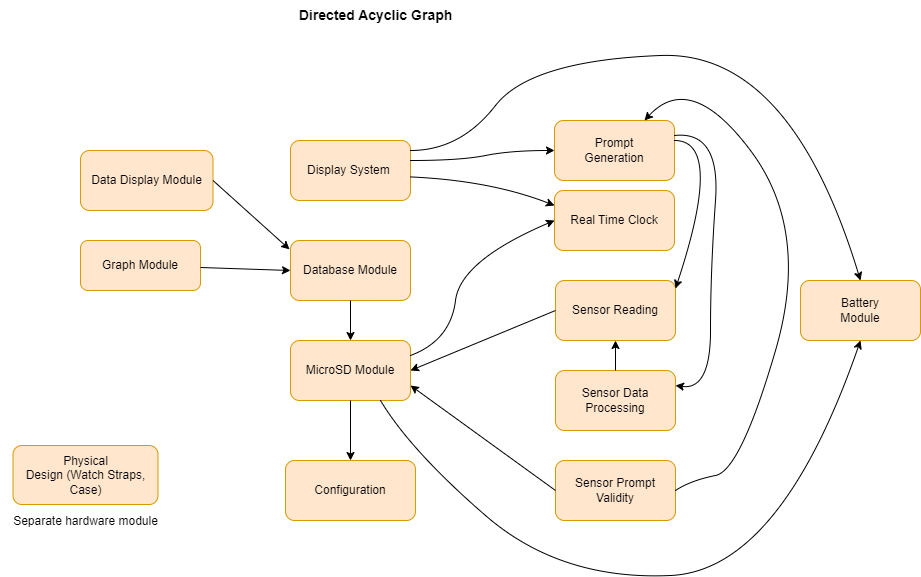
\includegraphics[width=\textwidth]{DAG.png}
  \caption{Use hierarchy among modules}
  \label{FigUH}
\end{figure}

%\section*{References}

\bibliographystyle {plainnat}
\bibliography{../../../refs/References}


\end{document}